\section{Présentation de la méthodologie}

Ce projet de grande envergure s’étale sur une durée de 12 semaines durant lesquelles des rendus intermédiaires seront effectués. Cela permet de pouvoir suivre l’avancement du travail et des différentes étapes de ce dernier. Il s’inscrit dans un processus méthodologique bien précis, découpé en grandes phases elles-mêmes découpées en sous-phases. Cette méthodologie est essentielle car elle suit une logique de conception centrale pour la bonne réalisation de ce projet. \\

Le figure suivant décrit ces différentes phrases :

\begin{figure}[H]
    \label{fig-LABEL-DE-LA-FIGURE}
    \noindent\makebox[\textwidth]{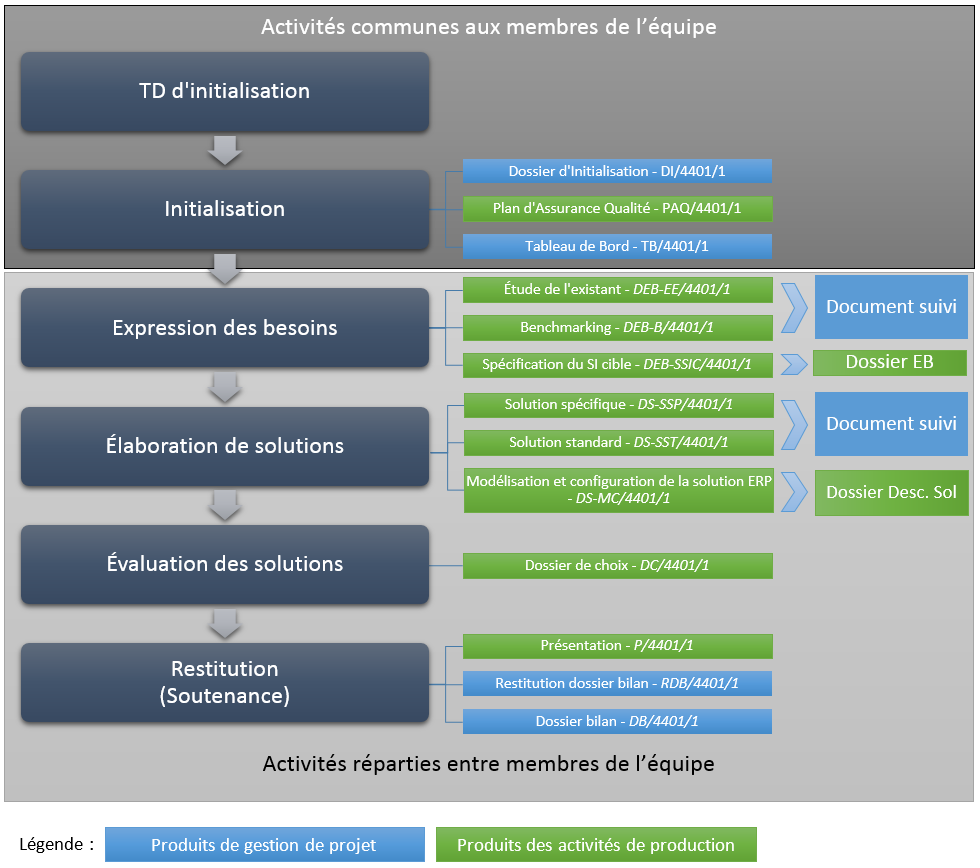
\includegraphics[width=17cm]{figures/processus-pld.png}}
    \caption{Schéma récapitulatif du processus global du projet}
\end{figure}

\section{Détail par phase}

\subsection{Phase 1 : Initialisation du projet}

Cette première phase occupe les deux premières semaines du projet. Elle consiste en la réalisation des premiers rendus intermédiaires, c’est-à-dire le PAQ et le dossier d’initialisation. De ce fait, les objectifs sont principalement de déterminer les éléments importants à mettre en place dès le début du projet pour la bonne cohérence des différents documents organisationnels que nous allons produire. \\

Il faut aussi avoir une première connaissance et définition du métier et du périmètre fonctionnel sur lequel porte ce projet, et donc sur lequel portera toute l’étude, permettant une transition vers l’expression des besoins. Cette première étape permet au client de prendre connaissance de la manière avec laquelle nous procédons, notre organisation et toute autre information importante relative à la manière dont le projet sera conduit.

\subsection{Phase 2 : Expression des besoins}

Cette phase est la phase la plus importante. Elle permet de comprendre les différents aspects, à la fois fonctionnels, mais aussi techniques, du métier et du besoin qui a mené à la demande à laquelle ce projet tente de répondre. En effet, la première étape de cette phase est d’abord de se plonger au c\oe{}ur du métier et des processus qui sont actuellement mis en place au sein de l’entreprise, afin d’en comprendre toutes les facettes. Nous devons parvenir à identifier l’ensemble des objets et le domaine d’application, ainsi qu’à comprendre et maîtriser ces derniers. À l’aide d’outils de modélisation ARIS tels que ARIS Architect, disponible sur la plateforme ARIS mise à notre disposition par le client, nous pourrons identifier, formaliser et détailler ces processus et les acteurs impliqués sous forme de diagrammes BPM. \\

Dans un deuxième temps il sera question de comprendre les nouveaux besoins du client par rapport à l’existant. Cette étape pourra se dérouler sous forme de groupes de travail ou de réunions.

\subsection{Phase 3 : Élaboration des solutions}

Suite à l’expression des besoin dans laquelle nous aurons identifié l’existant en détail ainsi que les différentes attentes client vis-à-vis du nouveau SI en projet, il nous faudra définir plusieurs solutions à proposer en réponse au besoin et exigences du client. Deux solutions sont à définir, une reposant sur un ERP, et une autre plus classique, dans la continuité du SI existant.

\subsection{Phase 4 : Recommandations sur les solutions}
 
Dans cette phase, notre travail consistera en la critique des différentes solutions proposées par l’équipe et l’apport de conseils au client. L’idée étant de rendre la prise de décision plus aisée pour le client en lui fournissant une critique constructive basée sur des critères précis et éventuellement définis avec ce dernier.

\subsection{Phase 4 : Restitution}

Phase essentielle et primordiale du projet, c’est le moment où nous devrons soumettre nos solutions au client. Il s'agira alors de  réussir à convaincre le client tout en montrant les différentes aspects de notre projet et le soin qui y a été apporté.
